\documentclass[12pt,a4paper]{article}
\usepackage[utf8x]{inputenc}
\usepackage{ucs}

\usepackage[T1]{fontenc}
\usepackage{amsmath}
\usepackage{amsfonts}
\usepackage{amssymb}
\usepackage{graphicx}
\usepackage[margin=0.5in]{geometry}

\author{Dorottya Cserpan}

\title{Single Cell Kernel Current Source Density}
\begin{document}
\maketitle

\section{Introduction}

\section{Overview of Relevant Current Source Density Methods (CSD)}
The relationship between the current sources and the generated potentials is given by the Poisson-equation:

%For this we have to use 
\begin{equation}
 \sigma \nabla^2 \Phi(\mathbf{r},t )= -C(\mathbf{r},t),
\label{eq:poisson1}
\end{equation} 
where $\sigma$ is the electrical conductivity of the extracellular medium, $\Phi$ is the 
extracellular potential, $\mathbf{r}$ refers to the position, and 
%\begin{equation}
$C(\mathbf{r},t)= \sum_{n=1}^N I_n (t) \delta^3(\mathbf{r}-\mathbf{r_n}) $
%\end{equation}
 is the current source density, the summation goes over all point sources,the position of the $n^{th}$ current source is $\mathbf{r_n}$ . There are several methods which use different assumptions for solving the above mentioned equation. 

\subsection{Traditional CSD}
The traditional CSD method \cite{Nicholson} uses the recorded extracellular potential from a laminar electrode, which is placed perpendicularly (z direction) to the layers of the cortex. Based on this setup and assuming that the layers are endless and homogeneous, the current source densities of each layer can be given:
\begin{equation}
C(z_j)= - \sigma \frac{\Phi(z_j+h)-2\Phi(z_j)+\Phi(z_j-h)}{h^2}
\end{equation}
 where $z_j$ is the position along the z-axis of the $j^{th}$ electrode and h is the inter-electrode distance.
\subsection{Kernel CSD}
The kCSD method \cite{DanielW} extends the applicability of the traditional CSD by enabling to calculate the current source densities at arbitrary positions by using kernel methods. 


  
\subsection{Spike CSD}
The Spike CSD \cite{Soma} aims to calculate the current source distribution of single neurons. This requires the estimation of the cell-electrode distance and a simplified model of the shape of the neuron. Separating the potential patterns generated by different neurons is a crucial point. A key for doing this is the separation based on the clustering of potential shapes generated by the action potentials, which are like fingerprints: different for every neuron. The limitation of this model is the simplified morphology of the model and the low spatial resolution.

\section{The  kCSD method for single neurons (ksCSD)}
Motivation: new imaging technology with high spatiotemporal distribution
Biological relevance:   Fluorescent dyes enable such reconstruction after the recording was done.

%In this method we mix the main ideas of the previous two methods, that is  the calculation of current source distribution of single neurons by using kernel methods. The main advantages of this method is the more accurate spatial resolution, but for this the morphology of the cell is needed. Fluorescent dyes enable such reconstruction after the recording was done. In order to test the method simulations with different parameters were carried out.


The extension of kernel methods for single cells
The CSD distribution can be expressed as the sum of the $M$ sources: 
\begin{equation}
C (\textbf{x})= \sum_{j=i}^M a_j \tilde{b}_j(\textbf{x})
\end{equation}

$\tilde{b}$ is the source function correlated to the segments of the neuron,$a_j$ is a multiplication constant.




%\begin{equation}
%\tilde{b}
%= a
%\left\{
%\begin{array}{l l} 
%1 & \quad \textsl{if \bold} 2\\
%0 & \quad 2\\
%\end{array}
%\right
%\end{equation}

The generated potential by the $\tilde{b_i}$ is denoted as  $b_i$, and the connection is made by the $A$ linear operator.

\begin{equation}
\label{eq:bfun}
b_i (x,y,z)= A \tilde{b}_i (x,y,z)= \frac{1}{4 \pi \sigma} \iiint 
\frac{ \tilde{b}_i (x',y',z')}{\sqrt{(x-x')^2+(y-y')^2+(z-z')^2}} dx' dy' dz'
\end{equation}

There is an infinite number of basis function we could use, one of the most common one is the Gaussian source function:
\begin{equation}
\label{eq:basisfun}
\tilde{b}_i (x,y,z) = e^{- \frac{(x-x_i)^2+(y-y_i)^2+(z-z_i)^2}{R^2}}
\end{equation}
Here $R$ is the double of the variance of the Gaussian function. The connection between the current sources densities and potentials is introduced by the $A$ operator($A: \tilde{F}\rightarrow F$)
\begin{equation}
\Phi(\textbf{x})= A C(\textbf{x}) =  \sum_{i}^M a_i b_i (\textbf{x})
\end{equation}
 where $b_i = A \tilde(b)_i$.
 
% The space of the sources is:
 
 
 
% In case of point sources:
 
%\begin{equation}
%\tilde{b}_j (\textbf{x}) = \delta((\textbf{x},\textbf{x}_{j}))
%\end{equation}
The detailed derivation of this method can be found in the \cite{DanielW}. reference, due to the length limitation it's not detailed here.
To determine the CSD distribution in arbitrary positions($x$), the following kernel functions were introduced:

\begin{equation}
K(\textbf{x}_k,\textbf{x}_l)= \sum_{i=1}^M b_i (\textbf{x}_k) b_i (\textbf{x}_l)
\end{equation} 
 
\begin{equation}
\tilde{K}(\textbf{x}_k,\textbf{y}_l)= \sum_{j=1}^M b_ (\textbf{x}_k) \tilde{b}_j (\textbf{y}_l) 
\end{equation} 
 
Using the simulated or measured extracellular potentials ($V$) and assuming $\tilde{K}$ is invertible the solution for $C$ is straightforward.
 \begin{equation}
 C(\textbf{x})=\tilde{\textbf{K}}^T(\textbf{x})  
 \tilde{\textbf{K}}^{-1} \textbf{V}
 \end{equation}



\subsection{ Linear source solution }
%As linear current distributions are used for the reconstruction, the method can be reduced to 1 dimension. For we assume that the cell can be reconstructed from lines.
While reconstructing the shape of the neuron first we needed to identify the branching points and the branches. After that given on the morphology information each branch were estimated by a spline. The basis functions were distributed along these curves uniformly. The current source density distributions were estimated along these splines as well. 



\begin{itemize}
\item 
\end{itemize}
The curves in the 3D space can be parametrized with variable $t$. 
%Let's say we have two points $A (x_a,y_a,z_a), B (x_b,y_b,z_b)$ in the space and we want to get the equation of the line which goes through these. 


%\begin{equation}
\begin{eqnarray}
\displaystyle x &=& f_x(t)  \nonumber \\
\displaystyle y &=& f_y(t)  \\
\displaystyle z &=& f_z(t)  \nonumber 
\end{eqnarray}
%\end{equation}


Writing the \ref{eq:basisfun}. equations in this formalism:
\begin{equation}
\tilde{b}_i (t') = e^{- \frac{(t' - t_i)^2}{R^2}}
\end{equation}
where both $t,t_i \in \left[ 0, d \right] $ are parameters on the same branch which has a length of $d$. 
%\begin{equation}
%\tilde{b}_i (t) = e^{- \frac{(x_a + (x_b - x_a) t -x_i)^2+(y_a+(y_b-y_a)t-y_i)^2+( z_a+(z_b-z_a)t-z_i)^2}{R^2}}
%\end{equation}
Writing the \ref{eq:bfun}. equations in this formalism:


\begin{equation}
b_i (x,y,z)= A \tilde{b}_i (t')= \frac{1}{4 \pi \sigma} \int 
\frac{ \tilde{b}_i (t')}{\sqrt{(x-x'(t))^2+(y-y'(t))^2+(z-z'(t))^2}} dt'
\end{equation}



%\begin{equation}
%\begin{align}
%b_i (x,y,z) &= 
%\frac{1}{4 \pi \sigma} \int 
%\frac{ e^{- \frac{(x_a + (x_b - x_a) t -x_i)^2+(y_a+(y_b-y_a)t-y_i)^2+( z_a+(z_b-z_a)t-z_i)^2}{R^2}}}{\sqrt{(x-x_a + (x_b - x_a) t)^2+(y- y_a+(y_b-y_a)t )^2+(z-z_a+(z_b-z_a)t)^2}} \\
%&\sqrt{(x_b-x_a)^2 +(y_b-y_a)^2+(z_b-z_a)^2} dt
%\end{align}
%\end{equation}

\subsection{Simulations}

Different distribution used
\begin{itemize}
\item test distributions (cosinus with different frequency, Gaussians with different widths)
\item ballstick neuron with current injected to the soma (spatiotemporal current distribution)
\item ballstick neuron with synapsis (spatiotemporal current distribution)
\end{itemize}



\subsubsection{Test distributions on a line}
For developing the basic properties of the method and finding the best parameters for a specific setup we used some simple distributions \ref{fig:distribution} to make estimations.

\begin{figure}[h]
\centering
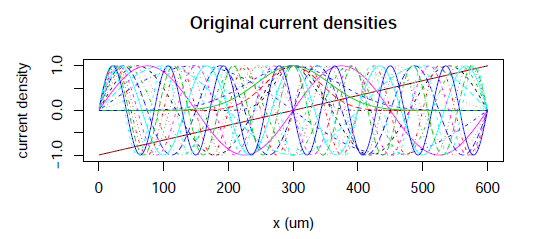
\includegraphics[width= 10 cm]{plots/distributions.png}
\caption{The test distributions}
\label{fig:distribution}
\end{figure}




The shematic figure of the simulational setup is show on \ref{fig: test_setup}.


\begin{figure}[h]
\centering
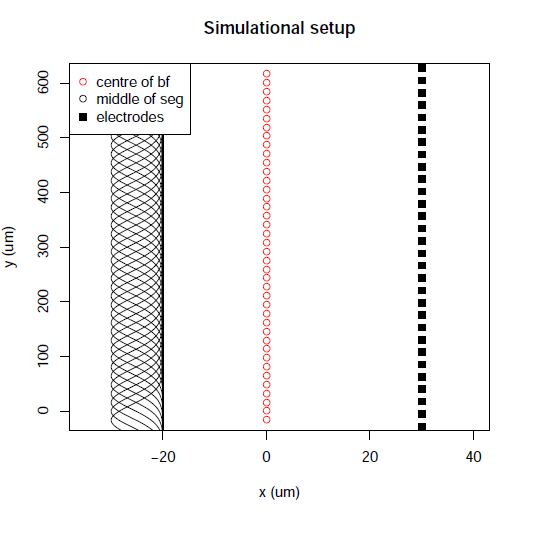
\includegraphics[width= 10 cm]{plots/setup_test.png}
\caption{The setup for the test simulation}
\label{fig: test_setup}
\end{figure}
In the simulations all the current density distributions were aligned on a $600 \mu m$line, which is parallel to the electrode shank. The resolution of the method is mainly depending on the number of electrodes used for the recording, here to cases of using 16 and 32 electrodes are shown. Also the number of basis functions applied, the type and width of basis function and the cell-to-electrode distance were modified. The basis functions were uniformly distributed. The parameters for this simulations were set in a way that it is similar to the simulation of the ballstick modell.
%For testing I used the bs_1D_130509test2.Rnw files for the simulation, the bs_130509for_test2.sh for running the simulation and the plotting_test.R, to plot the results....


%figures with cos basis functions
\begin{figure}[h]
%\centering
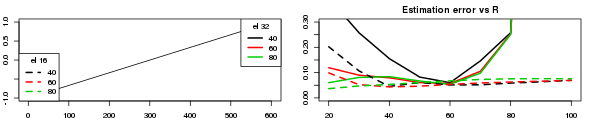
\includegraphics[width=15cm]{plots/error_Rtest_cos_patt1_el_both.png}
\caption{Type of basis function: cos, cell to el dist: 30 um, R:20-100, el nb: 16,32 , number of basis function: 40,60,80}
\label{fig:error_cos0}
\end{figure}


\begin{figure}[h]
%\centering
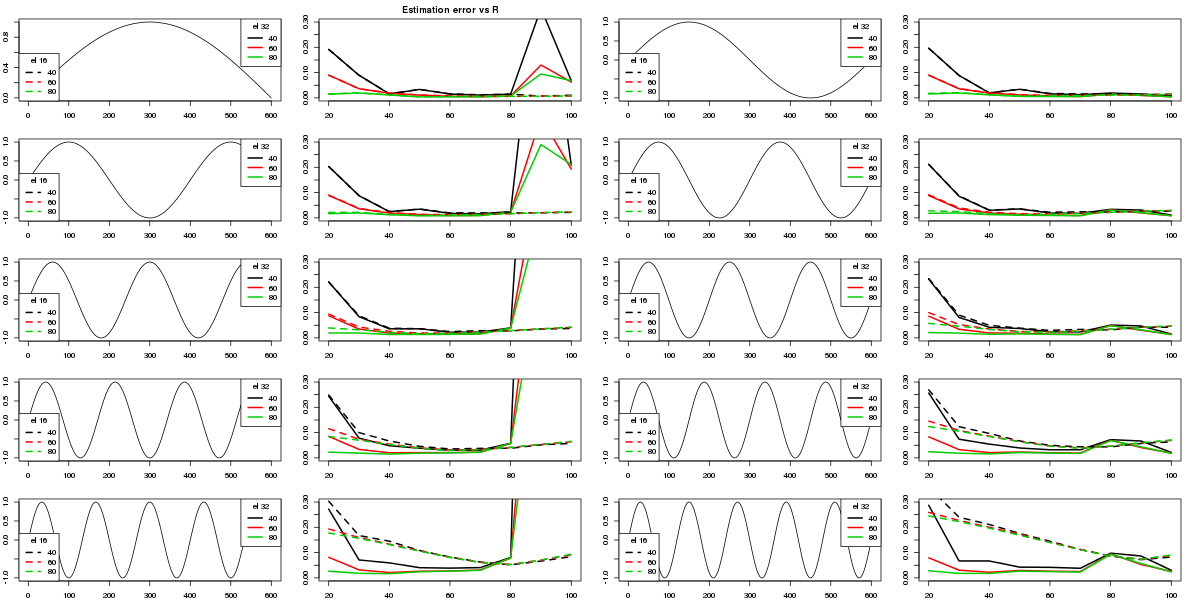
\includegraphics[width=15cm]{plots/error_Rtest_cos_patt3_12_el_both.png}
\caption{Type of basis function: cos, cell to el dist: 30 um, R:20-100, el nb: 16,32 , number of basis function: 40,60,80}
\label{fig:error_cos}
\end{figure}

\begin{figure}[h]
%\centering
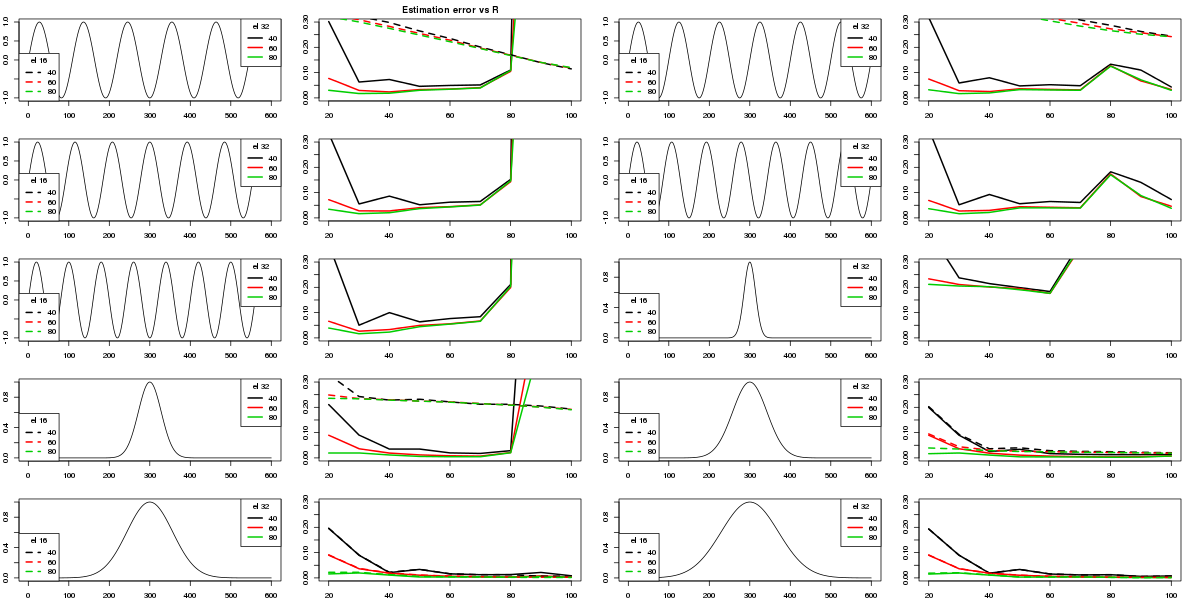
\includegraphics[width=15cm]{plots/error_Rtest_cos_patt13_22_el_both.png}
\caption{Type of basis function: cos, cell to el dist: 30 um, R:20-100, el nb: 16,32 , number of basis function: 40,60,80}
\label{fig:error_cos2}
\end{figure}
%figures with gaussian basis functions


\begin{figure}[h]
%\centering
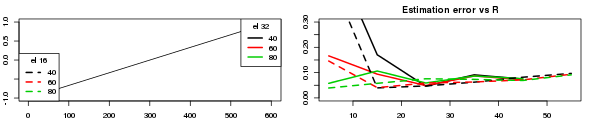
\includegraphics[width=15cm]{plots/error_Rtest_gauss2_patt1_el_both.png}
\caption{Type of basis function: gauss, cell to el dist: 30 um, R:20-100, el nb: 16,32 , number of basis function: 40,60,80}
\label{fig:error_gauss0}
\end{figure}


\begin{figure}[h]
%\centering
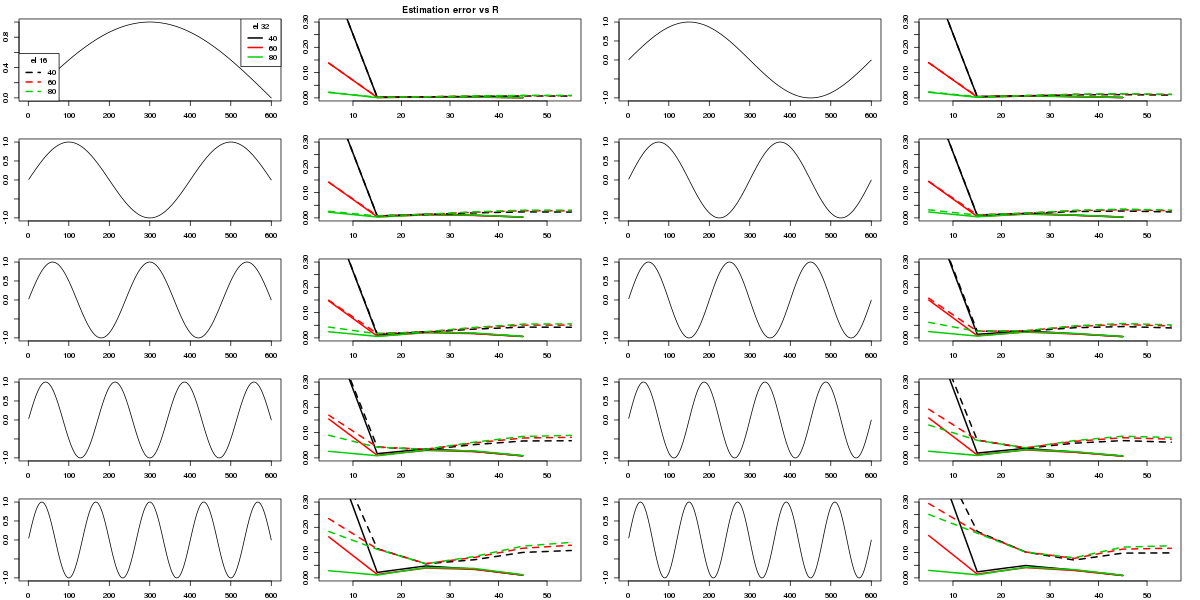
\includegraphics[width=15cm]{plots/error_Rtest_gauss2_patt3_12_el_both.png}
\caption{Type of basis function: gauss, cell to el dist: 30 um, R:20-100, el nb: 16,32 , number of basis function: 40,60,80}
\label{fig:error_gauss}
\end{figure}

\begin{figure}[h]
%\centering
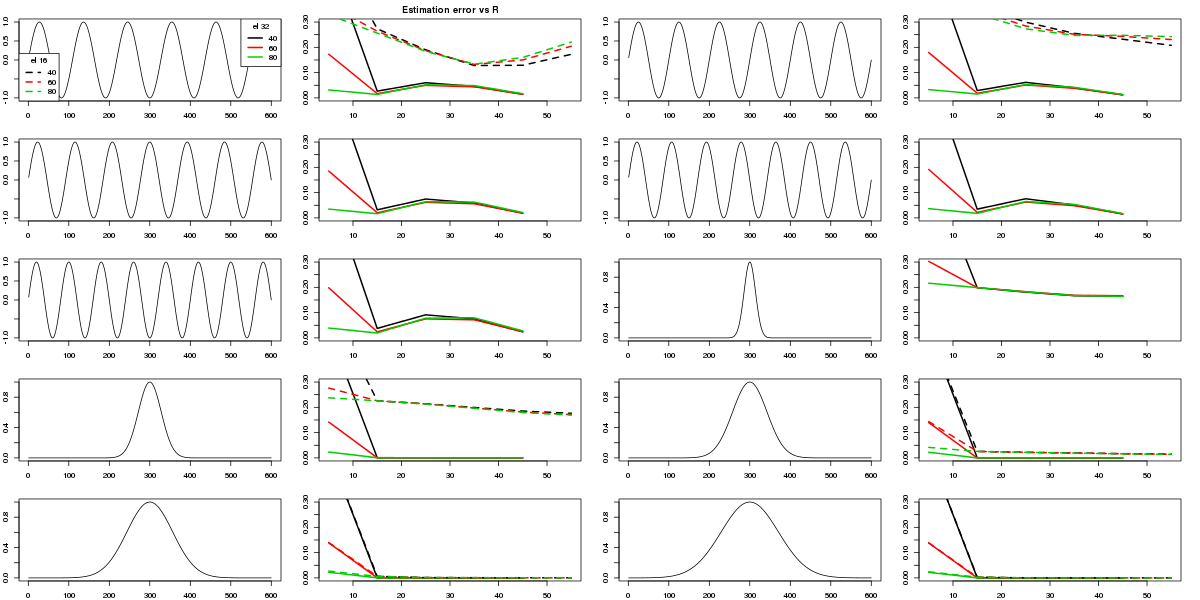
\includegraphics[width=15cm]{plots/error_Rtest_gauss2_patt13_22_el_both.png}
\caption{Type of basis function: gauss, cell to el dist: 30 um, R:20-100, el nb: 16,32 , number of basis function: 40,60,80}
\label{fig:error_gauss2}
\end{figure}

Conclusion

Generally increasing the number of the used basis functions improves the accuracy of the method to a certain limit.The resolution of the method is limited by the number of recording sides. Even though it is possible to calculate the current sources in arbitrary many points, the result is a smoothed curve. For some range of width of the basis function using more of them means more overlapping, which results poorer accuracy. The accuracy is slightly depending on the type of the basis function used, the Gaussian basis function seem to perform better in general.



\subsubsection{Ballstick morphology}


\textbf{Stimulation of the soma}
The simulation of extracellular potential of a ballstick neuron model was done by using LFPy \cite{LFPy}, which is a tool designed to calculate the extracellular potential of model neurons. An excitatory current lasting 100 ms injected into the soma-ball assured the continuous action potential generation.  The 1 dimensional neuron model was aligned parallel to the electrode, similar to the test simulations. The diameter of the soma is 18.8 um. 



\subsection{Cells with more complex morphology}
The main advantage of this method compared to the sCSD methods is the possibility to calculate the current distributions on branches as well. The distribution of the basis function on the branching morphology is though a challenge.

Basic assumptions:
\begin{itemize}
\item the shape of the branches is estimated by a spline
%\item at the branching points all the current densities are averaged out the solve the barrier conditions
\item the sources are evenly distributed
\item the branches are handled separately, they are independent from each other, an other solution would be to create overlapping sources
\end{itemize}

Ideas:
\begin{itemize}
\item Should we rather use volume sources instead? It will be impossible to trace al the branches...
\item What spatial distribution is necessary? 
\end{itemize}

Usually the morphology of the cell is very complex with lot's  of branches and the distribution of this method cannot reach this spatial accuracy. Let's say that the total length of all the segments is 10 000 $\mu$m. In this case if we have 100 recording sites, the spatial distribution will be around 100 um, which compared to the length and with of the cell is not that good, in this case some other approach might works better. One kind of solution for this could be the chopping off the branches with a diameter less than a certain value. This relies on the assumption that the amplitude of the membrane currents on these branches are much smaller???.


 The other problem is, that in tissue usually signals originating no further than 60 $mu$m from the electrode can be distinguished from the noise (reference!!!), which is typically  less, than the width of the neuron.

Properties of the multielectrode array:
1D or 2D

%\subsection{Parameters} 
%In the calculation shown here the following parameters were used (Fig. 1.):

%\begin{itemize}
%\item Number of electrodes: 10
%\item Number of source functions: 15
%\item Width of source functions: 70 um
%\item Sigma of Gaussian: 0.2
%\item Shift of overlapping of base functions: 25 um
%\item Cell to electrode distance: 30 um
%\end{itemize}
 
%$\tilde{b}$ is the source function correlated to the segments of the neuron,$a_j$ is a multiplication constant.



%\begin{equation}
%\tilde{b}
%= a
%\left\{
%\begin{array}{l l} 
%1 & \quad \textsl{if \bold} 2\\
%0 & \quad 2\\


\end{document}